\documentclass[
  11pt,
  a4paper,
  % titlepage,
]{article}

\title{Artificial Intelligence and Machine Learning}
\author{Martin de Spirlet}
\date{}

% Set document geometry
\usepackage[
  a4paper,
  margin = 1in,
  % showframe,
]{geometry} % Flexible and complete interface to document dimensions

% Set default font family to default sans-serif font
\renewcommand{\familydefault}{\sfdefault}

\usepackage{amsmath} % AMS mathematical facilities for LaTeX
\usepackage{amssymb} % TeX fonts from the American Mathematical Society
\usepackage{booktabs} % Publication quality tables in LaTeX
\usepackage{caption} % Customising captions in floating environments
\usepackage[inline,shortlabels]{enumitem} % Control layout of itemize enumerate description
\usepackage{graphicx} % Enhanced support for graphics
\usepackage[skip=\glueexpr\baselineskip\relax]{parskip} % Layout with zero \parindent non-zero \parskip
\usepackage[onehalfspacing]{setspace} % Set space between lines % setspace must be loaded before hyperref
\usepackage{titlesec} % Select alternative section titles

\PassOptionsToPackage{hyphens}{url}\usepackage{hyperref} % Extensive support for hypertext in LaTeX % hyperref loaded by pdfx

% Set list parameters (using enumitem package)
\setlist{nosep}

% Set section break command (using package titlesec)
\newcommand{\sectionbreak}{\clearpage}

% Define command for typesetting a mathematical function
\newcommand{\function}[3][]{\mathrm{#2}#1\!\left( #3 \right)}

% Increase penalty for widows and orphans (maximum 10000)
\widowpenalty = 10000
\clubpenalty = 10000

\begin{document}

\pagenumbering{gobble}

\maketitle

\vspace*{\fill}

\begin{table}[htp]
  \centering
  \begin{tabular}{rrl}
    \toprule
    Week & Unit & Title \\
    \midrule
    1 & 1 & Supervised Learning \\
      & 2 & Regression \\ [1ex]
    2 & 3 & Logistic Regression (Classification) \\
      & 4 & Neural Networks, Hyperparameters and Metrics \\ [1ex]
    3 & 5 & Na\"{i}ve Bayes \\ [1ex]
    4 & 6 & Decision Trees \\
      & 7 & \( k \)-Nearest Neighbours \\ [1ex]
    5 & 8 & Uninformed Search \\
    \bottomrule
  \end{tabular}
\end{table}

\vspace*{\fill}
\addvspace{1in}

\clearpage

\pagenumbering{arabic}

\section{Supervised Learning}
\subsection{Machine Learning}

The focus of \emph{machine~learning} is the study and development of computational models capable of improving their performance with experience and acquiring knowledge by themselves.
Learning algorithms can be classified into three broad groups.
\begin{description}
  \item[Unsupervised] learning algorithms, such as the \( k \)-means algorithm, classify input data based on certain inherent properties of that data.
  \item[Supervised] learning algorithms, such as regression, logistic regression and neural networks, learn trends from annotated data in order to make predictions about previously unseen data.
  \item[Reinforced] learning algorithms learn how to achieve specific tasks in predefined environments based on rewards.
\end{description}

\subsection{Terminology and Notation}

\subsubsection{Independent and Dependent Variables}

\emph{Independent variables} take on different values based on the environment.
\emph{Dependent variables} take on values based on other variables (usually independent variables).
Dependent variables \emph{depend} on independent variables.

Dependent variables can take on continuous or discrete values.
The prediction of continuous values is known as \emph{regression}.
The prediction of discrete values or \emph{classes} is known as \emph{classification}.

For both regression and classification, a supervised learning model consists of
\begin{itemize}
  \item a hypothesis function,
  \item a cost function, and
  \item a weight update function that uses the partial differential of the cost function.
\end{itemize}

\subsubsection{Training and Test Data}

The \emph{training data} used in supervised learning are \emph{annotated} with the values of the dependent variable \( y \) for each vector \( \boldsymbol{X} \) of independent variables.
Each training datum \( i \) is of the form \( \left( \boldsymbol{X}^{(i)}, y^{(i)} \right) \).
Thus, the training data may be represented in the form
\begin{equation*}
  \left( \boldsymbol{X}^{(1)}, y^{(1)} \right), \left( \boldsymbol{X}^{(2)}, y^{(2)} \right), \ldots, \left( \boldsymbol{X}^{(N)}, y^{(N)} \right)
\end{equation*}
For each of the \( N \) training inputs \( \boldsymbol{X}^{(i)} \), the corresponding output is \( y^{(i)} \).

The \emph{test data} is an independent set of annotated data on which the trained model is tested.
While it shares the characteristics of the training data, it contains different elements.

\subsubsection{Hypothesis Function}

The \emph{hypothesis function} \( \function[_{\boldsymbol{w}}]{h}{\boldsymbol{X}} \) predicts the output \( y \) that corresponds to the input \( \boldsymbol{X} \)\@.
For regression, the general form of the hypothesis function is
\begin{equation*}
  \function[_{\boldsymbol{w}}]{h}{\boldsymbol{X}} = w_0 + w_1 x_1 + w_2 x_2 + \ldots +  w_k x_k
\end{equation*}
where \( k \) is an arbitrary number of terms (not necessarily the number of elements in \( \boldsymbol{X} \)), and each term \( x \) may be the product of any combination of elements in \( \boldsymbol{X} \)\@.

The hypothesis function is parametrised by a vector of \emph{weights} \( \boldsymbol{w} \).
The purpose of a supervised learning algorithm is to find the values of these weights for which the hypothesis function best fits the training data.

\subsubsection{Cost Function}

The accuracy of a hypothesis function is measured using a \emph{cost function}.
When the cost function is at its minimum, the hypothesis function is said to \emph{fit} the data well.

\subsubsection{Gradient Descent}

The differential of a function gives the equation of the slope of the function.
The point where the slope is zero is a stationary point (minimum, maximum or point of inflection) of the function.
Since the determination of the minimum of the cost function may not always be trivial, an algorithm is used.
\emph{Gradient~descent} is an algorithm that uses the partial derivative of the cost function to find the values of the weights for which the cost function is at its minimum.


\section{Regression}
\subsection{Univariate Linear Regression}

\subsubsection{Hypothesis Function}

\emph{Univariate linear regression} is used to train a model that assumes a linear relationship between a single independent variable \( x \) and a dependent variable \( y \).
The hypothesis function for univariate linear regression is of the form
\begin{equation*}
  \function[_{\boldsymbol{w}}]{h}{x} = w_{0} + w_{1} x
\end{equation*}
This is a linear equation in which \( w_{0} \) represents the \( y \)-intercept and \( w_{1} \) represents the gradient.
The aim of univariate linear regression is to find the specific values of these parameters such that the line given by the hypothesis function fits the training data.

\subsubsection{Cost Function}

The loss functions typically used for regression are \emph{absolute~deviation} (or \emph{L1~loss}) and \emph{squared~error} (or \emph{L2~loss}).
For each training sample \( i \), the L1~loss of the prediction is the absolute difference between the actual value \( y^{(i)} \) and the predicted value \( \function[_{\boldsymbol{w}}]{h}{x^{(i)}} \) of the dependent variable.
\begin{equation*}
  \left\lvert y^{(i)} - \function[_{\boldsymbol{w}}]{h}{x^{(i)}} \right\rvert
\end{equation*}
The corresponding L2~loss is the square of this difference.
\begin{equation*}
  \left( y^{(i)} - \function[_{\boldsymbol{w}}]{h}{x^{(i)}} \right)^{2}
\end{equation*}

Both loss functions return a positive value so that the loss for each sample can be summed meaningfully, regardless of whether the prediction is greater than or less than the actual value.
L2~loss is the more commonly used loss function, since squaring the difference causes a prediction further from the actual value to incur a greater penalty.

The corresponding cost functions give the average loss over all \( m \) training samples.
\begin{equation*}
  \frac{1}{m} \sum_{i=1}^{m} \left\lvert y^{(i)} - \function[_{\boldsymbol{w}}]{h}{x^{(i)}} \right\rvert
\end{equation*}
\begin{equation*}
  \frac{1}{m} \sum_{i=1}^{m} \left( y^{(i)} - \function[_{\boldsymbol{w}}]{h}{x^{(i)}} \right)^{2}
\end{equation*}

\subsubsection{Gradient Descent}

The gradient~descent algorithm progressively updates the weights that parametrise the hypothesis function in order to minimise its cost.
The general form of gradient~descent is
\begin{enumerate}
  \item while the model has not \emph{converged} (the cost is not minimal),
  \begin{enumerate}
    \item for each training sample \( i \),
    \begin{enumerate}
      \item calculate the derivative of the loss on \( i \), and
      \item update all weights \( w \) using this value of the derivative.
    \end{enumerate}
  \end{enumerate}
\end{enumerate}

Each complete iteration over all training elements is known as an \emph{epoch}.
The model has converged when the weights parametrise the hypothesis function such that its cost is minimal.
One simple way to check for convergence is to wait until the costs of consecutive epochs are very small.

In the case of univariate linear regression using the derivative of L2~loss, the gradient descent algorithm is
\begin{enumerate}
  \item while the model has not \emph{converged} (the cost is not minimal),
  \begin{enumerate}
    \item for each training sample \( i \),
    \begin{align*}
      \text{Let}\, &{L^{\prime}}_{2}^{(i)} = y^{(i)} - \function[_{\boldsymbol{w}}]{h}{x^{(i)}} \\
      \text{Let}\, &w_{1} = w_{1} + \alpha \cdot {L^{\prime}}_{2}^{(i)} \cdot x^{(i)} \\
      \text{Let}\, &w_{0} = w_{0} + \alpha \cdot {L^{\prime}}_{2}^{(i)}
    \end{align*}
  \end{enumerate}
\end{enumerate}

The parameter \( \alpha \) is the \emph{learning rate} and represents the size of each step towards the correct values of \( w \).
If the learning rate is too large, the cost may begin to rise, causing gradient descent to fail.

\subsection{Multivariate and Non-Linear Regression}

\subsubsection{Hypothesis Functions}

\emph{Multivariate linear regression} is used to train a model that assumes a linear relationship between a vector of independent variables \( \boldsymbol{X} \) and a dependent variable \( y \).
The hypothesis function for multivariate linear regression is of the form
\begin{equation*}
  \function[_{\boldsymbol{w}}]{h}{\boldsymbol{X}} = w_{0} + w_{1} x_{1} + w_{2} x_{2} + \ldots
\end{equation*}
A term \( x^{(j)}_{i} \) refers to the \( i \)th input attribute of the \( j \)th training sample.

\emph{Univariate non-linear regression} is used to train a model that assumes a non-linear relationship between a single independent variable \( x \) and a dependent variable \( y \).
The hypothesis function for univariate non-linear regression is of the form
\begin{equation*}
  \function[_{\boldsymbol{w}}]{h}{x} = w_{0} + w_{1} x^{1} + w_{2} x^{2} + \ldots
\end{equation*}

\emph{Multivariate non-linear regression} is used to train a model that assumes a non-linear relationship between a vector of independent variables \( \boldsymbol{X} \) and a dependent variable \( y \).
The hypothesis function for multivariate non-linear regression is of the form
\begin{equation*}
  \function[_{\boldsymbol{w}}]{h}{\boldsymbol{X}} = w_{0} + w_{1} x_{1} + w_{2} x_{2} + w_{3} x_{1} x_{2} + w_{4} x_{1}^{2} + w_{5} x_{2}^{2} + \ldots
\end{equation*}

\subsubsection{Cost Function}

The cost functions used for univariate linear regression do not change for multivariate or non-linear regression.
Only the hypothesis function \( \function[_{\boldsymbol{w}}]{h}{\boldsymbol{X}} \) used to predict the dependent variable \( y \) changes.
The general L2~cost function is
\begin{equation*}
  \frac{1}{m} \sum_{i=1}^{m} \left( y^{(i)} - \function[_{\boldsymbol{w}}]{h}{\boldsymbol{X}^{(i)}} \right)^{2}
\end{equation*}

\subsubsection{Gradient Descent}

The general gradient~descent algorithm also applies to multivariate and non-linear regression.
The only changes are the hypothesis function \( \function[_{\boldsymbol{w}}]{h}{\boldsymbol{X}} \) and the number of weights \( w \) to be updated.
The general gradient~descent algorithm using the derivative of L2~loss is
\begin{enumerate}
  \item while the model has not \emph{converged} (the cost is not minimal),
  \begin{enumerate}
    \item for each training sample \( j \),
    \begin{equation*}
      \text{Let}\, {L^{\prime}}_{2}^{(j)} = y^{(j)} - \function[_{\boldsymbol{w}}]{h}{\boldsymbol{X}^{(j)}} \\
    \end{equation*}
    \begin{enumerate}
      \item for each weight \( w_{i} \) and its corresponding \( x \)-term \( \function[_{i}]{f}{\boldsymbol{X}^{(j)}} \) in the hypothesis function,
      \begin{equation*}
        \text{Let}\, w_{i} = w_{i} + \alpha \cdot  {L^{\prime}}_{2}^{(j)} \cdot \function[_{i}]{f}{\boldsymbol{X}^{(j)}}
      \end{equation*}
    \end{enumerate}
  \end{enumerate}
\end{enumerate}


\section{Logistic Regression (Classification)}
\subsection{Binary Classification}

\emph{Logistic~regression} is used as a form of \emph{binary~classification}.
Instead of training a model to predict a trend, logistic regression is used to train a model that predicts whether a sample belongs to a discrete class.
A logistic regression model produces a continuous output value between zero and one that is interpreted as the probability that the sample belongs to the class.

\subsection{Hypothesis and Activation Functions}

The hypothesis function for logistic regression is better known as an \emph{activation function}.
One common class of activation function is the \emph{logistic function}, which is itself a \emph{sigmoid function}.
The basic logistic function \( \function{g}{z} \) returns a value in the finite domain from zero to one.
\begin{equation*}
  \function{g}{z} = \frac{1}{1 + e^{-z}}
\end{equation*}
\begin{equation*}
  \begin{cases}
    \begin{aligned}
      0.5 < \function{g}{z} &< 1 & \text{when } z &> 0 \text{,} \\
      \function{g}{z} &= 0.5 & \text{when } z &= 0 \text{,} \\
      0 < \function{g}{z} &< 0.5 & \text{when } z &< 0 \text{.}
    \end{aligned}
  \end{cases}
\end{equation*}

Thus, hypothesis functions that use the logistic function \( \function{g}{z} \) as an activation function can be expressed in the form
\begin{equation*}
  \function[_{\boldsymbol{w}}]{h}{\boldsymbol{X}} = \function{g}{\boldsymbol{w}^{\mathrm{T}} \boldsymbol{X}}
\end{equation*}

The hypothesis function for univariate linear logistic regression is of the form
\begin{equation*}
  \function[_{\boldsymbol{w}}]{h}{x} = \function{g}{w_{0} + w_{1} x}
\end{equation*}

The hypothesis function for multivariate linear logistic regression is of the form
\begin{equation*}
  \function[_{\boldsymbol{w}}]{h}{\boldsymbol{X}} = \function{g}{w_{0} + w_{1} x_{1} + w_{2} x_{2} + \ldots}
\end{equation*}

The hypothesis function for univariate non-linear logistic regression is of the form
\begin{equation*}
  \function[_{\boldsymbol{w}}]{h}{x} = \function{g}{w_{0} + w_{1} x + w_{2} x^{2} + \ldots}
\end{equation*}

The hypothesis function for multivariate non-linear logistic regression is of the form
\begin{equation*}
  \function[_{\boldsymbol{w}}]{h}{\boldsymbol{X}} = \function{g}{w_{0} + w_{1} x_{1} + w_{2} x_{2} + w_{3} x_{1} x_{2} + w_{4} x_{1}^{2} + w_{5} x_{2}^{2} + \ldots}
\end{equation*}

\subsection{Decision Boundary}

The \emph{decision boundary} separates samples that do not belong to the class from samples that do.
Data with \( N \) input attributes may be plotted in \( N \)-dimensional space.
The decision boundary is an object that can be expressed in \( N - 1 \) dimensions, separates samples in \( N \)-dimensional space and extends infinitely far.
For example, data with two input attributes can be plotted on a plane and separated by line.
Classes for which the decision boundary is a straight or flat object, such as a point, line, plane or hyperplane, are said to be \emph{linear~separable}.
These classes are predicted by linear logistic regression models.

The decision boundary is formed by all possible points where the hypothesis function is equal to a specific value.
Using the basic logistic function, this value is typically \( \function{g}{0} = 0.5 \).
Samples for which \( \function{g}{\boldsymbol{w}^{\mathrm{T}} \boldsymbol{X}} \geq 0.5 \) are predicted to belong to the class.
Samples for which \( \function{g}{\boldsymbol{w}^{\mathrm{T}} \boldsymbol{X}} < 0.5 \) are predicted not to belong to the class.

\subsection{Cost Function}

The cost function evaluates the accuracy of the hypothesis function with respect to a set of training samples.
The derivative of the cost function is used in the gradient~descent algorithm to update the weights that parametrise the hypothesis function.
For gradient~descent to work, the cost function must be convex.
The cost functions used in linear regression cannot be used to evaluate the accuracy of a sigmoid function, as the resultant combination is not convex, and the gradient descent algorithm is likely to converge on a local minimum, rather than the global minimum.

The loss of a single sample in logistic regression is given by
\begin{multline*}
  - y^{(i)} \log \function[_{\boldsymbol{w}}]{h}{\boldsymbol{X}^{(i)}} - \left( 1 - y^{(i)} \right) \function{\log}{1 - \function[_{\boldsymbol{w}}]{h}{\boldsymbol{X}^{(i)}}} \\
  = \begin{cases}
    - y^{(i)} \log \function[_{\boldsymbol{w}}]{h}{\boldsymbol{X}^{(i)}} & \text{when } y^{(i)} = 1 \text{,} \\
    - \left( 1 - y^{(i)} \right) \function{\log}{1 - \function[_{\boldsymbol{w}}]{h}{\boldsymbol{X}^{(i)}}} & \text{when } y^{(i)} = 0 \text{.}
  \end{cases}
\end{multline*}
This expression has the following useful properties.
\begin{itemize}
  \item Since the actual value \( y^{(i)} \) of the dependent variable can only be zero or one, only one term of the expression contributes to the loss for a single sample.
  \item When the actual value \( y^{(i)} \) is zero and the prediction \( \function[_{\boldsymbol{w}}]{h}{\boldsymbol{X}^{(i)}} \) is zero, the loss is zero.
  \item When the actual value \( y^{(i)} \) is zero and the prediction \( \function[_{\boldsymbol{w}}]{h}{\boldsymbol{X}^{(i)}} \) tends towards one, the loss tends towards infinity.
  \item When the actual value \( y^{(i)} \) is one and the prediction \( \function[_{\boldsymbol{w}}]{h}{\boldsymbol{X}^{(i)}} \) is one, the loss is zero.
  \item When the actual value \( y^{(i)} \) is one and the prediction \( \function[_{\boldsymbol{w}}]{h}{\boldsymbol{X}^{(i)}} \) tends towards zero, the loss tends towards infinity.
\end{itemize}

The corresponding cost over all \( m \) training samples is given by
\begin{equation*}
  - \frac{1}{m} \sum_{i=1}^{m} \left( y^{(i)} \log \function[_{\boldsymbol{w}}]{h}{\boldsymbol{X}^{(i)}} + \left( 1 - y^{(i)} \right) \function{\log}{1 - \function[_{\boldsymbol{w}}]{h}{\boldsymbol{X}^{(i)}}} \right)
\end{equation*}

\subsection{Gradient Descent}

The general gradient~descent algorithm also applies to logistic regression.
The only changes are the hypothesis function \( \function[_{\boldsymbol{w}}]{h}{\boldsymbol{X}} \) and the number of weights \( w \) to be updated.
The general gradient~descent algorithm for logistic regression is
\begin{enumerate}
  \item while the model has not \emph{converged} (the cost is not minimal),
  \begin{enumerate}
    \item for each training sample \( j \),
    \begin{equation*}
      \text{Let}\, {L^{\prime}}_{2}^{(j)} = y^{(j)} - \function[_{\boldsymbol{w}}]{h}{\boldsymbol{X}^{(j)}} \\
    \end{equation*}
    \begin{enumerate}
      \item for each weight \( w_{i} \) and its corresponding \( x \)-term \( \function[_{i}]{f}{\boldsymbol{X}^{(j)}} \) in the hypothesis function,
      \begin{equation*}
        \text{Let}\, w_{i} = w_{i} + \alpha \cdot  {L^{\prime}}_{2}^{(j)} \cdot \function[_{i}]{f}{\boldsymbol{X}^{(j)}}
      \end{equation*}
    \end{enumerate}
  \end{enumerate}
\end{enumerate}


\section{Neural Networks, Hyperparameters and Metrics}
\subsection{Neural Networks}

\subsubsection{Motivation}

A hypothesis function that is both non-linear and highly multivariate will have a large number of weights.
Optimising a large number of weights using gradient descent is impractical.
In these situations, it is useful to break the problem down into smaller linear regression problems.

\subsubsection{Structure of a Neural Network}

A \emph{neural~network} comprises many \emph{linear logistic regression units} (also known as \emph{logits}, \emph{perceptrons}, or more generally \emph{neurons} or \emph{nodes}).
The nodes are grouped into an \emph{input} layer, one or more \emph{hidden} layers, and an \emph{output} layer.
Typically, each node in a layer is an input to every node in the following layer.
The number of nodes in the input layer is one more than the number of input attributes in the data.
The additional node is known as a \emph{bias}, and holds the constant value of one, which corresponds to the implicit constant term that is multiplied by the weight \( w_{0} \) to give the \( y \)-intercept.
Bias nodes exist to allow functions that do not pass through the origin to be captured.

Each logistic regression unit has its own weight vector \( \boldsymbol{w} \), and applies a linear hypothesis function \( \function[_{\boldsymbol{w}}]{h}{\boldsymbol{X}} \) to its inputs \( \boldsymbol{X} \).
The output node is also a logistic regression unit with its own weights and a bias input node in the preceding hidden layer.

The total cost of a neural network is the sum of the linear (typically L2) costs of its output nodes.
Finding the derivative of the cost function to use in gradient descent is non-trivial.
An algorithm such as \emph{backpropagation} is used to implement automatic differentiation and to update the weights.

\emph{Deep~learning} is a machine learning technique that uses a neural~network with multiple hidden layers.

\subsubsection{Multinomial Classification}

In a \emph{multinomial} or \emph{multiclass} neural network, each output node produces the probability that a sample belongs to a particular class.
This is known as a \emph{one-versus-all} probability; the probability that a sample belongs to a particular class is the complement of the probability that it belongs to any other class that may be predicted by the model.
Since each output probability describes a different class, there is no constraint that the sum of the output probabilities is one.
Nevertheless, the probability associated with one class is useful for predicting the probabilities associated with other classes.
For example, a high probability that a sample belongs to one class suggests that the probability of the sample belonging to another class is low.
Typically, the predicted class is that returned by the \emph{softargmax} function --- a function that normalises a vector of probabilities and returns the index of the greatest.

\subsubsection{Training Data and Test Data}

\emph{Training data} is used to create a model.
\emph{Test data} is used evaluate the model after it has been trained.
Both training data and test data are annotated so that the accuracy of predictions may be measured.
The test data must be separate from the training data to ensure the model is tested on unseen samples.
Testing the model on the data on which it is trained would produce meaningless results.
Nevertheless, it is important that the test data has similar characteristics, such as probability distribution, to the training data.
A model can only make a reliable prediction on data similar to what it has already encountered.
In other words, regression is used to interpolate between known data.

\subsubsection{Overfitting}

A model that fits the training data too closely may make poor predictions on unseen data.
While the training data is similar to unseen data, they are not exactly the same.
\emph{Overfitting} can be identified when the performance on the training data increases over consecutive epochs while the performance on the test data reduces.
Overfitting is the result of a model that is more complex than required.
\emph{Complexity} is determined by the number of non-linear terms in the hypothesis function and the magnitude of the weights associated to them.

\subsubsection{Regularisation}

\emph{Regularisation} diminishes the effects of high-order polynomial terms in a hypothesis function by penalising any high weights associated to them.
This helps to prevent overfitting.

For example, \emph{L2 regularisation} adds a weighted sum of the squares of the weights to the cost of the hypothesis.
\begin{equation*}
  \text{Let cost} = \text{cost} + \lambda \sum_{i=1}^{m} w_{i}^{2}
\end{equation*}

More generally, regularisation can be achieved by
\begin{itemize}
  \item including regularisation penalties for each logistic regression unit,
  \item dropout --- bypassing certain nodes (typically half) during training to prevent the network from learning the training data too well, or
  \item reducing the network depth.
\end{itemize}

\subsubsection{Activation Functions}

Each logistic regression unit applies an activation function to the sum of its weighted inputs.
Sigmoid functions are only one class of activation function.
Others include the \emph{hyperbolic tangent} (\emph{tanh}) and \emph{rectified linear unit} (\emph{ReLU}).

\subsection{Hyperparameters}

The performance of a neural network is governed by a number of parameters, such as the number of nodes and layers, the method of regularisation, the activation function and the learning rate.
These are known as \emph{hyperparameters}.

\emph{Hyperparameter optimisation} --- the process of selecting the correct combination of hyperparameters --- can be critical to the success of a project.
It can also be incredibly expensive in terms of time and computational resources.
One method of hyperparameter optimisation is \emph{grid~search}, which involves testing all possible combinations of hyperparameters in order to find the most performant.

It is possible for a combination of hyperparameters to fit the test data so well that it does not work on a new set of data.
To prevent this, hyperparameter combinations may be tested against another set of annotated data --- \emph{validation data}.

\subsection{Metrics}

The \emph{accuracy} metric is simply the proportion of predictions that are correct.
While this is intuitive, it fails to penalise false positives, particularly when the distribution of classes in the test data is not equal.
For example, a hypothesis function that predicts all samples belong to a particular class regardless of their independent attributes is not very useful.
Yet, when tested on a set of test data in which \( 90\% \) of all samples belong to that class, it will achieve an accuracy of \( 90\% \).

Usually, a better metric to use is the \emph{F1~score}.
This is the harmonic mean of \emph{precision} --- the proportion of selected samples that are relevant --- and \emph{recall} --- the proportion of relevant samples that are selected.


\section{Na\"{i}ve Bayes}
\subsection{Probability Theory}

\subsubsection{Random Variables}

Variables in probability theory are known as \emph{random variables}.
The \emph{domain} of a random variable is the set of values it can take.
For regression, the output domain is, in general, the set of real numbers \( \mathbb{R} \)\@.
For classification, the output domain is a finite set of ordinals or categories.

\subsubsection{Probability Distributions}

A probability distribution \( \function{P}{X = x} \) is a function that maps a possible value \( x \) of a random variable \( X \) in domain \( \mathcal{X} \) to the probability of observing it.
When the name of the variable \( X \) is obvious or irrelevant, it may be omitted.
The sum of all probabilities in a probability distribution is one.
\begin{equation*}
  \sum_{x \in \mathcal{X}} \function{p}{x} = 1
\end{equation*}

An \emph{unconditional} or \emph{prior} probability distribution describes the probabilities of different observations in the absence of additional information.

A \emph{conditional} or \emph{posterior} probability distribution describes the probabilities of different events given some evidence.
For example, the probability of an event \( Y \) given an event \( X \) is expressed as
\begin{equation*}
  \function{P}{Y \vert X}
\end{equation*}

A \emph{joint} probability distribution describes the probability of two events occurring together.
For example, the probability of an events \( X \) and \( Y \) occurring together is expressed as
\begin{equation*}
  \function{P}{X, Y} = \function{P}{X \text{ and } Y} = \function{P}{X \land Y}
\end{equation*}

For the purposes of machine learning, it can be assumed that a process generates data (training, test or other) based on an unknown joint probability distribution \( \function{P}{\boldsymbol{X}, Y} \) between a vector of independent input variables \( \boldsymbol{X} \), each in a domain \( \mathcal{X} \), and a dependent output variable \( Y \) in the domain \( \mathcal{Y} \).

\subsubsection{Probability Density Functions}

A \emph{continuous variable} can take an infinite number of values between any two limits.
A \emph{probability density function} describes the relative likelihood of a continuous variable taking a value between two limits.
The area under the curve of a probability density function \( \function{f}{X} \) between two values \( a \) and \( b \) of a variable \( X \) represents the probability of the variable falling between those values.
\begin{equation*}
  \function{P}{a \leq X \leq b} = \int_{a}^{b} \function{f}{X}\, \mathrm{d} X
\end{equation*}

Since there are an infinite number of values that a continuous variable can take, the relative likelihoods of all values do not sum to one.
Instead, the area under the curve of the probability density function is one.

\subsection{Bayes' Theorem}

A joint probability distribution \( \function{P}{\boldsymbol{X}, Y} \) can be expressed as
\begin{equation*}
  \function{P}{\boldsymbol{X}, Y} = \function{P}{\boldsymbol{X}} \function{P}{Y \vert \boldsymbol{X}} = \function{P}{Y} \function{P}{\boldsymbol{X} \vert Y}
\end{equation*}
Bayes' theorem states that
\begin{equation*}
  \function{P}{X \vert Y} = \frac{\function{P}{X} \function{P}{Y \vert X}}{\function{P}{Y}}
\end{equation*}

In terms of machine learning, the joint probability of observing a vector of input attributes \( \boldsymbol{a} \) with an output class \( c \) is
\begin{equation*}
  \function{p}{\boldsymbol{a}, c} = \function{p}{\boldsymbol{a}} \function{p}{c \vert \boldsymbol{a}} = \function{p}{c} \function{p}{\boldsymbol{a} \vert c}
\end{equation*}
Thus, the probability of observing a particular class \( c \) given a vector of input attributes \( \boldsymbol{a} \) is given by
\begin{equation*}
  \function{p}{c \vert \boldsymbol{a}} = \frac{\function{p}{c} \function{p}{\boldsymbol{a} \vert c}}{\function{p}{\boldsymbol{a}}}
\end{equation*}

A machine learning model could learn the unconditional probabilities \( \function{p}{\boldsymbol{a}} \) and \( \function{p}{c} \), and the conditional probability \( \function{p}{\boldsymbol{a} \vert c} \), and use them to make predictions based on Bayes' theorem.
Learning the probabilities is a simple case of keeping track of the frequencies of different input and output values, and their combinations.

\subsection{Normalisation}

The denominator \( \function{p}{\boldsymbol{a}} \) acts as a normalisation factor that ensures the probabilities for all classes \( c \), given input attributes \( \boldsymbol{a} \), sum to one.
\begin{equation*}
  \sum_{c \in \mathcal{Y}} \function{p}{c \vert \boldsymbol{a}} = \sum_{c \in \mathcal{Y}} \frac{\function{p}{c} \function{p}{\boldsymbol{a} \vert c}}{\function{p}{\boldsymbol{a}}} = 1
\end{equation*}
Since the normalisation factor is the same for every class, it can be extracted as follows.
\begin{equation*}
  \function{p}{c \vert \boldsymbol{a}} = \alpha \function{p}{c} \function{p}{\boldsymbol{a} \vert c}, \quad \alpha = \beta^{-1}, \quad \beta = \sum_{c \in \mathcal{Y}} \function{p}{c} \function{p}{\boldsymbol{a} \vert c}
\end{equation*}
This notation is useful as the assumptions made by the na\"{i}ve Bayes model cause \( \function{p}{\boldsymbol{a}} \) not to work as a normalising factor.

\subsection{Na\"{i}ve Bayes for Categorical Independent Variables}

\subsubsection{Conditional Independence}

Bayes' theorem for \( n \) independent variables where \( n \geq 1 \) expands from
\begin{equation*}
  \function{p}{c \vert \boldsymbol{a}} = \alpha \function{p}{c} \function{p}{\boldsymbol{a} \vert c}
\end{equation*}
to
\begin{equation*}
  \function{p}{c \vert a_{1}, \ldots, a_{n}} = \alpha \function{p}{c} \function{p}{a_{1}, \ldots, a_{n} \vert c}
\end{equation*}

For large \( n \), the number of possible combinations of input variables, and, therefore, the number of rows to be maintained in a frequency table, become intractable.
Instead, na\"{i}ve Bayes classifiers assume that each independent variable \( X \) is conditionally independent of every other independent variable, given the dependent variable \( Y \).
Thus, a smaller, separate frequency table can be maintained for each independent variable, and it can be assumed that
\begin{equation*}
  \function{p}{a_{1}, \ldots, a_{n} \vert c} = \prod_{i=1}^{n} \function{p}{a_{i} \vert c}
\end{equation*}

Thus, the na\"{i}ve Bayes equation becomes
\begin{equation*}
  \function{p}{c \vert \boldsymbol{a}} = \alpha \function{p}{c} \prod_{i=1}^{n} \function{p}{a_{i} \vert c}, \quad \alpha = \beta^{-1}, \quad \beta = \sum_{c \in \mathcal{Y}} \left( \function{p}{c} \prod_{i=1}^{n} \function{p}{a_{i} \vert c} \right)
\end{equation*}

\subsubsection{Laplace Smoothing}

One problem with this basic na\"{i}ve Bayes approach is that if there are no observations for a particular attribute value \( a_{i} \), the probability \( \function{p}{a_{i} \vert c} \) is zero, and, therefore, the entire probability \( \function{p}{c \vert \boldsymbol{a}} \) of observing the class \( c \) given the attributes \( \boldsymbol{a} \) is also zero, regardless of the values of the other attributes.
Although there may be no samples with this combination of class and attributes in the training data, it cannot be assumed that the combination is impossible.

To solve this problem, the constant value of one can be added to the observation frequencies of every attribute for each class.
This is known as \emph{Laplace~smoothing}.
The smoothed frequencies are used to calculate the conditional probabilities \( \function{p}{a_{i} \vert c} \).
The original frequencies are used to calculate the unconditional probabilities \( \function{p}{c} \).

\subsection{Na\"{i}ve Bayes for Numeric Independent Variables}

Typically, na\"{i}ve Bayes adopts a \emph{Gaussian distribution} (also known as a \emph{normal distribution}) for each numeric independent variable.
The probability density function of a Gaussian distribution \( \function{\mathcal{N}}{\mu, \sigma^{2}} \) with mean \( \mu \) and variance \( \sigma^{2} \) is given by
\begin{equation*}
  \function{P}{X = a \vert \mu, \sigma^{2}} = \frac{1}{\sqrt{2 \sigma^{2} \pi}} e^{- \frac{\left( a - \mu \right)^{2}}{2 \sigma^{2}}}
\end{equation*}

The na\"{i}ve Bayes model can learn the values of the parameters \( \mu \) and \( \sigma^{2} \) for each numeric attribute \( a_{i} \), and use them to calculate the relative likelihoods \( \function{p}{a_{i} \vert c} \) to use in the na\"{i}ve Bayes equation.

The mean \( \mu \) and variance \( \sigma^{2} \) for an attribute given a particular class are calculated using the set of observed values \( V \) of the attribute for that class.
\begin{gather*}
  \mu = \frac{1}{\left\lvert V \right\rvert} \sum_{v \in V} v \\
  \sigma^{2} = \frac{1}{\left\lvert V \right\rvert - 1} \sum_{v \in V} \left( v - \mu \right)^{2}
\end{gather*}

\subsection{Combined Na\"{i}ve Bayes Approach}

The na\"{i}ve Bayes learning algorithm creates and, therefore, a na\"{i}ve Bayes model comprises
\begin{itemize}
  \item frequency tables with an without Laplace~smoothing for categorical independent variables, and
  \item tables of probability density function parameters for numeric independent variables.
\end{itemize}

Na\"{i}ve Bayes assumes conditional independence of independent variables and predicts the class with the greatest \( \function{p}{c \vert a_{i}, \ldots, a_{n}} \).
\begin{equation*}
  \function{p}{c \vert \boldsymbol{a}} = \alpha \function{p}{c} \prod_{i=1}^{n} \function{p}{a_{i} \vert c}, \quad \alpha = \beta^{-1}, \quad \beta = \sum_{c \in \mathcal{Y}} \left( \function{p}{c} \prod_{i=1}^{n} \function{p}{a_{i} \vert c} \right)
\end{equation*}
The unconditional probability \( \function{p}{c} \) is calculated using frequency tables without Laplace~smoothing.
For categorical independent variables, the unconditional probability \( \function{p}{a_{i} \vert c} \) is calculated using frequency tables with Laplace~smoothing.
For numeric independent variables, the relative likelihood \( \function{p}{a_{i} \vert c} \) is calculated using probability density functions using learnt parameters.

The advantages of the na\"{i}ve Bayes approach are that
\begin{itemize}
  \item it is fast --- only one pass through the data is needed to learn its parameters, and
  \item the relative probabilities computed by the approach are suitable for many applications, including text categorisation and medical diagnosis.
\end{itemize}

The disadvantages of the na\"{i}ve Bayes approach are that
\begin{itemize}
  \item it assumes conditional independence of independent variables,
  \item it assumes a probability distribution for numeric independent variables,
  \item it does not work very well for regression problems, although variations of na\"{i}ve Bayes do exist for regression.
\end{itemize}


\section{Decision Trees}
\subsection{Structure of a Decision Tree}

A \emph{decision~tree} is a predictive model with a tree-like structure.
An \emph{internal~node} specifies a test to be be carried out on a single input attribute, and has a branch to be followed for each possible outcome of the test.
A \emph{leaf~node} indicates the value of the output attribute.
A prediction is made by starting at the root node, performing the test indicated by the current node, and following the outcome branch, continuing until a leaf node is reached.
Irrelevant or redundant attributes do not appear on a tree.
The smaller a tree, the easier it is to understand.

Depending on the type of its output attribute, a decision~tree can be either a \emph{classification~tree} or a \emph{regression~tree}.
Input attributes can be numerical, categorical or ordinal.

\subsection{Construction of a Decision Tree}

\subsubsection{General Procedure}

Decision trees are constructed by recursively splitting nodes until certain termination criteria are met.
To construct a decision tree
\begin{enumerate}
  \item create a root node and split it on the input attribute that best separates the samples associated with it into different classes (the attribute is that which provides the greatest information~gain),
  \item create a node for each outcome branch, and
  \item continue splitting nodes using the same procedure.
\end{enumerate}
Splitting on a particular branch stops when
\begin{itemize}
  \item all samples associated with a node have the same output class --- the node is made a leaf node of that class,
  \item there are no further attributes on which to split the node, but not all samples associated with the node have the same output class --- the node is made a leaf node of the majority class, or
  \item there are no samples associated with the node --- the node is made a leaf node of the majority class of its parent node.
\end{itemize}

\subsubsection{Entropy}

\emph{Entropy} is a measure of the impurity of a set of training samples.
A set in which samples are distributed equally among classes is \emph{impure}.
Impurity corresponds to high entropy.
A set in which all samples belong to the same class is \emph{pure}.
Purity corresponds to low entropy.

The entropy of a set of samples \( S \) that can belong to either class~A or class~B is defined in terms of the proportion of samples \( p_{\mathrm{A}} \) that belong to class~A, and the proportion of samples \( p_{\mathrm{B}} \) that belong to class~B.
\begin{equation*}
  \function{\text{entropy}}{S} = - p_{\mathrm{A}} \log_{2} p_{\mathrm{A}} - p_{\mathrm{B}} \log_{2} p_{\mathrm{B}}
\end{equation*}

More generally, the entropy of a set of samples \( S \) that can belong to any class \( c \) in the set of classes \( K \) is given by
\begin{equation*}
  \function{\text{entropy}}{S} = - \sum_{c \in K} p_{c} \log_{2} p_{c}
\end{equation*}

\subsubsection{Information Gain}

\emph{Information~gain} is a reduction in entropy (an increase in purity).
For classification problems, the input attribute that best separates the training samples into different classes is that which provides the greatest information~gain.

The information~gain of splitting a set of samples \( S \) by an attribute \( A \) with domain \( \mathcal{A} \) is given by
\begin{equation*}
  \function{\text{infogain}}{S, A} = \function{\text{entropy}}{S} - \sum_{a \in \mathcal{A}} \frac{\left\lvert S_{a} \right\rvert}{\left\lvert S \right\rvert} \function{\text{entropy}}{S_{a}}
\end{equation*}
where \( S_{a} \) is the subset of samples of \( S \) whose attribute \( A \) has the value \( a \).

\subsubsection{Formal Algorithm}

The formal algorithm for constructing a decision tree from a set of training samples \( S \) is as follows.
\begin{enumerate}
  \item Create a root node for the tree and associate all samples \( S \) with it.
  \item If all samples belong to the same class, return the root node as the leaf node of that class.
  \item If there are no more input attributes on which to split, return the root node as a leaf node of the majority class of the samples \( S \)\@.
  \item Select the remaining attribute \( A \) that provides the greatest information~gain.
  \item For each value \( a \) of \( A \),
  \begin{enumerate}
    \item add a new branch below the root node that corresponds to \( A = a \),
    \item find the subset of samples \( S_{a} \) that correspond to \( A = a \),
    \item if \( S_{a} \) is empty, add a leaf node below this branch and assign to it the majority class of the samples \( S \),
    \item else run this algorithm using \( S_{a} \) as \( S \) and add the resulting subtree below this branch.
  \end{enumerate}
  \item Return the tree starting from the root node.
\end{enumerate}

\subsection{Application of Decision Trees}

The main advantage of a decision tree is that it is easy to visualise and interpret.
Nevertheless, decision trees can grow very large even though they eliminate redundant and irrelevant attributes.
They can also vary significantly when trained on different sample sets.

Decision trees are suitable for problems in which input attributes are discrete (categorical or ordinal), and an interpretable model is required.
Decision trees have been used successfully to classify medical patients by their diseases, and equipment malfunctions by their causes.


\section{\texorpdfstring{\( k \)}{k}-Nearest Neighbours}
\subsection{Overview}

\( k \)\emph{-nearest neighbours} (\( k \)\emph{-NN}) is an intuitive approach that works by finding the training samples most similar to the new sample.
For classification, the \( k \)\emph{-NN} algorithm predicts the majority output class of the \( k \) nearest neighbours, where \( k \) is a positive integer and typically small.
For binary classification, an odd number is chosen for \( k \) to ensure that such a majority exists.
For regression problems, the algorithm predicts the average or median output attribute of the \( k \) nearest neighbours.

\subsection{Distance}

\subsubsection{Euclidean Distance}

Given an instance whose output attribute is to be predicted, the \( k \) nearest samples to the instance must be found using some distance metric on the input space.
Usually, Euclidean distance is used.
The Euclidean distance \( \function{d}{\boldsymbol{x}^{(i)} ,\boldsymbol{x}^{(j)}} \) between a sample input vector \( \boldsymbol{x}^{(i)} \) and a previously unseen input vector \( \boldsymbol{x}^{(j)} \) in \( N \)-dimensional space is given by
\begin{equation*}
  \begin{aligned}
    \function{d}{\boldsymbol{x}^{(i)} ,\boldsymbol{x}^{(j)}} &= \sqrt{\sum_{n=1}^{N} \left( x_{n}^{(j)} - x_{n}^{(i)} \right)^{2}} \\
    &= \sqrt{\left( x_{1}^{(j)} - x_{1}^{(i)} \right)^{2} + \left( x_{2}^{(j)} - x_{2}^{(i)} \right)^{2} + \ldots + \left( x_{N}^{(j)} - x_{N}^{(i)} \right)^{2}}
  \end{aligned}
\end{equation*}

\subsubsection{Normalisation}

One problem with calculating distance arises from the scales used to measure different numeric input attributes.
An input attribute whose values cover a large range will tend to contribute greatly towards the distance.
This means that changing the unit used to express the measurement of an input attribute can produce a vast difference in predictions, even though the meaning of the measurement has not changed.

A common solution is to normalise numeric input attributes such that their values always fall between zero and one, inclusive.
The normalised value \( {x^{\prime}}_{n}^{(i)} \) of the input attribute \( n \) of a sample \( \boldsymbol{x}^{(i)} \) is calculated using the minimum and maximum values of the attribute \( n \) as follows.
\begin{equation*}
  {x^{\prime}}_{n}^{(i)} = \frac{x_{n}^{(i)} - \min_{n}}{\max_{n} - \min_{n}}
\end{equation*}
If the global minimum and maximum possible values of the attribute are unknown, the sample minimum and maximum values are used.

\subsubsection{Ordinal and Categorical Input Attributes}

The possible values of an ordinal input attribute are mapped to equidistant values from zero to one, inclusive.
For an ordinal attribute with \( m \) possible values, this can be achieved by normalising the one-based index using a minimum of one and a maximum of \( m \).
The resulting values can be used to calculate Euclidean distances for the attribute.

The distance between two values of a categorical attribute \( n \) is zero if the values are equal, or one if they are not.
\begin{equation*}
  x_{n}^{(j)} - x_{n}^{(i)} = \begin{cases}
    0 & \text{if } x_{n}^{(i)} = x_{n}^{(j)}, \\
    1 & \text{otherwise}.
  \end{cases}
\end{equation*}

\subsection{Prediction}

Given training samples of the form \( \left( \boldsymbol{x}^{(i)}, y^{(i)} \right) \), a number of neighbours \( k \), and vectors of the minimum and maximum values for each attribute, the output attribute \( y^{(j)} \) of a new input vector \( \boldsymbol{x}^{(j)} \) is computed as follows.
\begin{enumerate}
  \item Update the minimum and maximum of each attribute using the values of \( \boldsymbol{x}^{(j)} \).
  \item Normalise each attribute of \( \boldsymbol{x}^{(j)} \) to produce a normalised vector \( {\boldsymbol{x}^{\prime}}^{(j)} \).
  \item For each training sample \( \left( \boldsymbol{x}^{(i)}, y^{(i)} \right) \),
  \begin{enumerate}
    \item normalise each attribute of \( \boldsymbol{x}^{(i)} \) to produce a normalised vector \( {\boldsymbol{x}^{\prime}}^{(i)} \),
    \item calculate the distance \( d \) between the normalised vectors \( {\boldsymbol{x}^{\prime}}^{(i)} \) and \( \boldsymbol{x}^{(j)} \), and
    \item store \( \left( d, y^{(i)} \right) \) in a data structure \( T \) sorted by \( d \) in ascending order.
  \end{enumerate}
  \item Return the mode (or average or median for regression) of \( y^{(i)} \) over the first \( k \) entries of \( T \)\@.
\end{enumerate}

\subsection{Summary}

The \( k \)-NN learning algorithm involves no real training.
It is a simple case of storing the training samples, and the minimum and maximum of each numeric input attribute.
This is a powerful approach when the number of training samples is small.
The prediction algorithm is also very intuitive; it finds the mode, average or median of the output attribute over the training samples most similar to the new sample.

The disadvantages of the \( k \)-NN approach are the large amount of memory required to store all the data, and the need to search all training samples to find the nearest neighbours --- both of which are major issues when the training set is large.
More efficient variants of the approach do exist.


\section{Uninformed Search}
\subsection{Problem Formulation}

\emph{Problem-solving} agents are able to search for a sequence of actions that result in a solution to a problem, which can then be applied to the problem to solve it.
This is known as the \emph{search~approach}.
An algorithm that searches for a solution to a \emph{search problem} is a \emph{search algorithm}.
An \emph{uninformed} search algorithm is given no information regarding states, other than the \emph{problem formulation}.

The elements of a problem formulation are
\begin{itemize}
  \item the initial state,
  \item the goal states,
  \item possible actions and their effects on states, and
  \item a cost function.
\end{itemize}

A goal state is a desired outcome of the problem.
A solution is a sequence of actions that lead from the initial state to a goal state.
The best solution is that with the lowest cost.
Typically, the cost of a solution is the sum of the costs of its actions.

A \emph{state~space graph} contains all the possible states of the problem.
It is implicitly defined by the initial state, and the possible actions and their effects on states.
A solution is a path through the state~space graph.
Some solutions are better than others.
It is not necessary to give the state~space graph as an input to a search algorithm.
Only the problem formulation is necessary.

\subsection{Search Trees}

A search tree is generated by a search algorithm in order to search for a solution.
Each node in the tree represents a state of the problem.
The root node represents the initial state of the problem.
Each connection between a pair of nodes corresponds to an action that transforms the state of the first node to the state of the second node.

In order to save memory, a search tree represents only the explored portion of the graph.
When a node has been expanded, it is often circled on the search tree diagram.
An expanded node is said to have been \emph{visited}.
The set of nodes in the tree that are available to be expanded is known as the \emph{frontier}.

Different search algorithms correspond to different ways of deciding which frontier node to visit next.
Breadth-first and depth-first searches are techniques that can be used when the costs of each action are the same.

\subsection{Breadth-First Search}

To perform a \emph{breadth-first} search
\begin{enumerate}
  \item visit the shallowest frontier node first, placing its children in the frontier, but
  \item do not place a child in the frontier if its corresponding state is represented by a node already in the frontier or the list of visited nodes.
  \item Stop searching when a goal node is placed in the frontier.
\end{enumerate}

Breadth-first search can be seen as a first-in, first-out (FIFO) algorithm.
The frontier is a FIFO queue, in which the earliest node is the first to be visited.

The search finds a solution for a given problem formulation.
The cost of the search is expressed in terms of its time and space complexity.
The cost of a solution is typically the sum of the costs of its actions.

A breadth-first search with a branch factor \( b \) (maximum number of children per node) and a shallowest goal depth \( d \) (where the root has a depth of zero) has the following properties.
\begin{itemize}
  \item It is complete --- as long as \( b \) is finite, the search is guaranteed to find a path to a goal state if one exists, or to terminate in failure otherwise.
  \item It is optimal --- the search is guaranteed to find the shortest path to a goal state, as long as all actions have the same cost.
  \item It has a worst-case space complexity of \( \function{O}{b^{d}} \).
  \item It has a worst-case time complexity of \( \function{O}{b^{d}} \).
\end{itemize}

The complexity \( \function{O}{b^{d}} \) means that in the worst case, the algorithm must generate and store \( b^{d} \) nodes, which may require a large amount of time and memory.
Thus, breadth-first search is not an efficient algorithm, and is not recommended for large problems.

\subsection{Depth-First Search}

To perform a \emph{depth-first} search
\begin{enumerate}
  \item visit the deepest frontier node first, placing its children in the frontier, but
  \item do not place a child in the frontier if its corresponding state is represented by a node already in the frontier or the list of visited nodes.
  \item Stop searching when a goal node is visited.
\end{enumerate}

Unlike a breadth-first search, a depth-first search does not stop until a goal node is visited, or all nodes are visited without reaching a goal node.
The rationale is to visit or expand every node in a branch until it cannot be expanded any further, or a goal node is found, before moving to another branch.

Depth-first search can be seen as a last-in, first-out (LIFO) algorithm.
The frontier is a LIFO stack, in which the latest node is the first to be visited.

A depth-first search has the following properties.
\begin{itemize}
  \item It is complete if the state space is finite --- if the state space is finite, the search is guaranteed to find a path to a goal state if one exists, or to terminate in failure otherwise
  \item It is not complete if the state space is infinite.
  \item It is not optimal --- it is not guaranteed to find the shortest path to a goal state.
  \item It has a worst-case space complexity of the order of the size of the state space.
  \item It has a worst-case time complexity of the order of the size of the state space.
\end{itemize}

A complexity of the order of the size of the state space means that in the worst case, the algorithm must generate and store the entire state space graph.

\subsection{Space-Saving Depth-First Search}

The standard depth-first search stores all previously visited states to ensure that the algorithm is complete when the state space is finite.
If previously visited states were not stored, it is possible that states may eventually be revisited, which may cause an infinite loop.

Memory could be saved without affecting completeness by only storing the nodes (and their unvisited siblings) in the path from the root to the current node.
For a search tree with a maximum depth of \( m \), this would have the following properties.
\begin{itemize}
  \item It has a reduced worst-case space complexity of \( \function{O}{b m} \).
  \item It has a reduced worst-case time complexity of \( \function{O}{b^{m}} \).
\end{itemize}

\subsection{Space-Saving Depth-Limited Search}

In order to guarantee that a depth-first search will terminate in a reasonable amount of time, a limit can be placed on the maximum search depth.
A \emph{depth-limited} search is a depth-first search to a maximum depth of \( L \), where the root node has a depth of zero.

To perform a depth-limited search
\begin{enumerate}
  \item visit the deepest frontier node first, placing its children in the frontier only if the depth \( d \) of the children is less than or equal to the depth limit \( L \), but
  \item do not place a child in the frontier if its corresponding state is represented by a node already in the stored frontier or the list of visited nodes.
  \item Stop searching when a goal node is visited.
\end{enumerate}

A space-saving depth-limited search with its shallowest goal at depth \( d \) has the following properties.
\begin{itemize}
  \item It is complete if \( d \leq L \).
  \item It is not optimal --- like the standard depth-first search, it is not guaranteed to find the shortest path to a goal state.
  \item It has a reduced worst-case space complexity of \( \function{O}{b L} \).
  \item It has a reduced worst-case time complexity of \( \function{O}{b^{L}} \).
\end{itemize}

Thus, the depth-limited search has the same or greater time complexity as a breadth-first search.

\begin{figure}[htp]
  \centering
  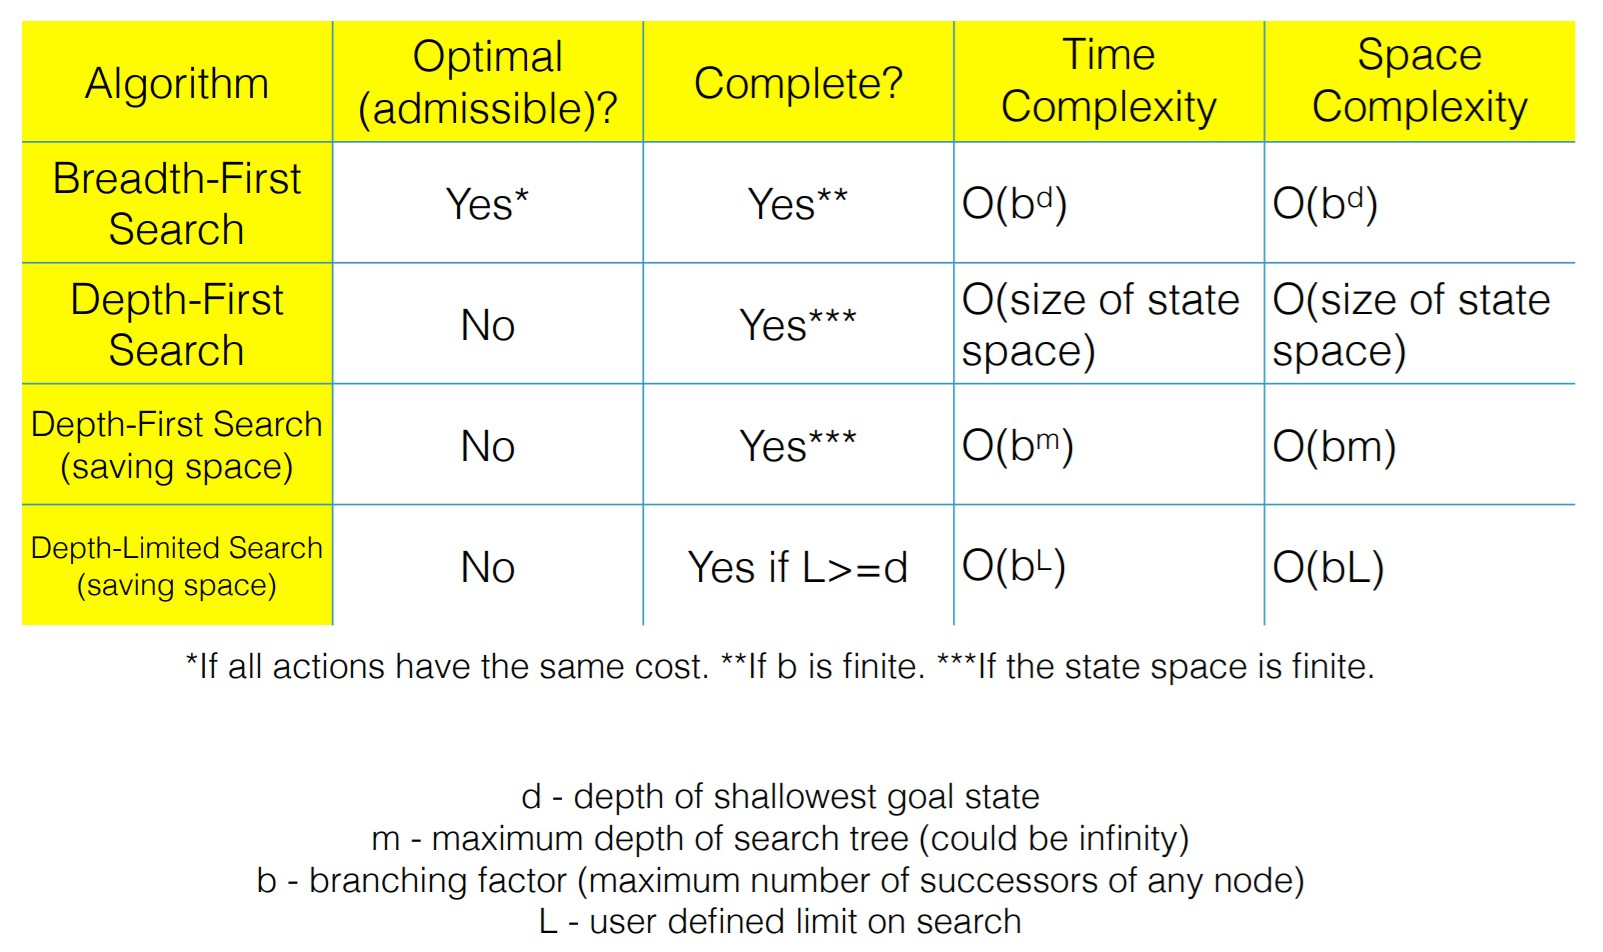
\includegraphics[width=0.8\textwidth]{unit-8/figures/uninformed-search-comparison.jpg}
  \caption*{Comparison of uninformed search algorithms.}
\end{figure}


\end{document}
